\documentclass{beamer}
\usetheme{metropolis}           % Use metropolis theme

\usepackage[english]{babel}

% Set page size and margins
% Replace `letterpaper' with `a4paper' for UK/EU standard size
%\usepackage[letterpaper,top=2cm,bottom=2cm,left=3cm,right=3cm,marginparwidth=1.75cm]{geometry}


%\usepackage{tikz}
%\usetikzlibrary{shapes.geometric, arrows}
%\tikzstyle{startstop} = [rectangle, rounded corners, minimum width=3cm, minimum height=1cm,text centered, draw=black, fill=red!30]
%\tikzstyle{io} = [trapezium, trapezium left angle=70, trapezium right angle=110, minimum width=3cm, minimum height=1cm, text centered, draw=black, fill=blue!30]
%\tikzstyle{process} = [rectangle, minimum width=3cm, minimum height=1cm, text centered, draw=black, fill=orange!30]
%\tikzstyle{decision} = [diamond, minimum width=3cm, minimum height=1cm, text centered, draw=black, fill=green!30]
%\tikzstyle{arrow} = [thick,->,>=stealth]




\pgfdeclarelayer{bg}
\pgfsetlayers{bg,main}


\usepackage{amsmath}
\usepackage{amsfonts}
\usepackage{graphicx}
%\usepackage[colorlinks=true, allcolors=cyan]{hyperref}
%\numberwithin{equation}{section}
%\usepackage{graphicx,wrapfig,lipsum,subfigure,sidecap,epsfig}
%\usepackage{caption}
%\usepackage{cancel}
%\usepackage{graphicx,subfigure,sidecap,epsfig} % Rouslan's subfig package
%\usepackage{soul}
%\usepackage[colorlinks=true,linkcolor=red]{hyperref}%
%\usepackage{mathtools}
%\usepackage{eqparbox}
%\usepackage{float} % \figure{}[H] IN PLACE VIEW
%\usepackage[capitalize]{cleveref} % smart references in one bracket
%\usepackage{hyperref}
%\usepackage{amssymb} % rightleft arrows
%\usepackage{cancel} % \cancelto{<value>}{expression} diagonally
%\usepackage[mathscr]{euscript}
%\DeclareSymbolFont{rsfs}{U}{rsfs}{m}{n}
%\DeclareSymbolFontAlphabet{\mathscrsfs}{rsfs}
%\usepackage{MnSymbol}

%%
%% CREF rules
%% Equation(s)
%\crefformat{equation}{#2Eq. (#1)#3}
%\crefrangeformat{equation}{#3Eqs. (#1)#4 to #5(#2)#6}
%\crefmultiformat{equation}{#2Eqs. (#1)#3}{ and #2(#1)#3}{, #2(#1)#3}{ and #2(#1)#3}
%\crefrangemultiformat{equation}{#3Eqs. ((#1))#4 to #5((#2))#6}{ and #3(#1)#4 to #5(#2)#6}{, #3(#1)#4 to #5(#2)#6}{ and #3(#1)#4 to #5(#2)#6}
%% Plural eqn
%\crefformat{pluralequation}{#2Eqs.~(#1)#3}
%% System
%\crefformat{system}{#2Sys.~(#1)#3}
%\crefrangeformat{system}{#3Sys. (#1)#4 to #5(#2)#6}
%\crefmultiformat{system}{#2Sys. (#1)#3}{ and #2(#1)#3}{, #2(#1)#3}{ and #2(#1)#3}
%\crefrangemultiformat{system}{#3Sys. ((#1))#4 to #5((#2))#6}{ and #3(#1)#4 to #5(#2)#6}{, #3(#1)#4 to #5(#2)#6}{ and #3(#1)#4 to #5(#2)#6}
%% Boundary conditions
%\crefformat{bc}{#2BC (#1)#3}
%\crefrangeformat{bc}{#3BCs (#1)#4 to #5(#2)#6}
%\crefmultiformat{bc}{#2BCs (#1)#3}{ and #2(#1)#3}{, #2(#1)#3}{ and #2(#1)#3}
%\crefrangemultiformat{bc}{#3BCs ((#1))#4 to #5((#2))#6}{ and #3(#1)#4 to #5(#2)#6}{, #3(#1)#4 to #5(#2)#6}{ and #3(#1)#4 to #5(#2)#6}
%% Steps
%\crefformat{step}{#2Step (#1)#3}
%\crefrangeformat{step}{#3Steps (#1)#4 to #5(#2)#6}
%\crefmultiformat{step}{#2Steps (#1)#3}{ and #2(#1)#3}{, #2(#1)#3}{ and #2(#1)#3}
%\crefrangemultiformat{step}{#3Steps ((#1))#4 to #5((#2))#6}{ and #3(#1)#4 to #5(#2)#6}{, #3(#1)#4 to #5(#2)#6}{ and #3(#1)#4 to #5(#2)#6}
%%diagram
%\crefformat{diagram}{#2Diagram (#1)#3}
%\crefrangeformat{diagram}{#3Diagrams (#1)#4 to #5(#2)#6}
%\crefmultiformat{diagram}{#2Diagrams (#1)#3}{ and #2(#1)#3}{, #2(#1)#3}{ and #2(#1)#3}
%\crefrangemultiformat{diagram}{#3Diagrams ((#1))#4 to #5((#2))#6}{ and #3(#1)#4 to #5(#2)#6}{, #3(#1)#4 to #5(#2)#6}{ and #3(#1)#4 to #5(#2)#6}



%\usepackage[sortcites=true]{biblatex} % biblatex DOEST WORK WITH LIVE TYPESETTER
\usepackage[nocompress]{cite}
%\bibliographystyle{ieeetr} % trash style mess up the order in bib



\graphicspath{{figures/}}

\title{Discrete streamfunction method for incompressible Navier-Stokes equation\\
(also known as Exact fractional step method)}
\date{\today}
\author{Rauan Kelesbekov}
\institute{University of Alberta}
\begin{document}
  \maketitle
  \section{Introduction}
  \begin{frame}{Introduction}
	\begin{figure}[H] % here - h, bottom - b, top - t
  	\centering{
  		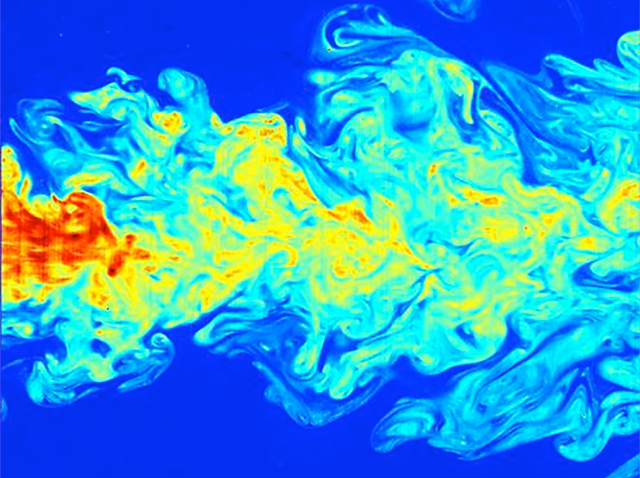
\includegraphics[width=0.55\paperwidth]{image1.png}
  	}
%  	\caption{Fluid flow}\label{fig:1}
	\end{figure}
	\end{frame}
  
  	\begin{frame}{Introduction}
  	Let $\boldsymbol{v}(x,y,t)=[u(x,y,t),v(x,y,t)]^T$ and $\boldsymbol{p}(x,y,t)$ be solutions to incompressible Navier-Stokes system of equations on 2D domain $\Omega$ with Dirichlet Boundary conditions on $\partial\Omega$.
	\begin{subequations}
	\label{eqs:NSE}
	\begin{align}
	\label{eqn:momentum-intro}
	\underbrace{\frac{\partial \boldsymbol{v}}{\partial t}}_{\text{transient}} 
		+ \underbrace{\boldsymbol{v} \cdot \nabla \boldsymbol{v}}_{\text{advective}} 
		&= \underbrace{-\nabla p}_{\text{pressure gradient}} 
		+ \underbrace{\epsilon \nabla \cdot \nabla \boldsymbol{v}}_{\text{viscous, Laplacian}}\quad\text{(momentum) in }\Omega\\
	\label{eqn:continuity}
	\nabla \cdot \boldsymbol{v} &= 0\quad\text{(continuity) in }\Omega,\\
%	\boldsymbol{v}(\xi(s,t)) &= \int_x\boldsymbol{v}(x)\delta(x - \xi)dx = \boldsymbol{v}_B(\xi(x,t)).
	\boldsymbol{v}&=\boldsymbol{v}(x,y,t)\quad\text{on }\partial\Omega
	\end{align}
	\end{subequations}
  \end{frame}
  
  \begin{frame}{Motivation}
	Stream function $\psi(x,y,t):\boldsymbol{v}=\nabla \times \psi$ of an incompressible two-dimensional flow:
	\begin{equation}
	\label{eqn:streamfunction}
		u = \frac{\partial \psi}{\partial y},\quad v=-\frac{\partial \psi}{\partial x}.
	\end{equation}
	Vorticity $\omega = \nabla \times \boldsymbol{v}$, in two-dimensional case (x-y-plane) the only non-zero component of $\omega$ is $z$, which leads to
	\begin{equation}
	\label{eqn:vorticity}
		\omega=- \frac{\partial u}{\partial y}+\frac{\partial v}{\partial x}.
	\end{equation}
  \end{frame}
  
  \begin{frame}{Motivation}
  \eqref{eqn:streamfunction} into \eqref{eqn:vorticity} leads to
	\begin{equation}
			\label{eqn:vorticity-stream}
			-\nabla ^2 \psi = \omega.
		\end{equation}
  Apply $(\nabla \times)$ to momentum. Since
	\begin{equation}
	\frac{\partial}{\partial y}\left(\frac{\partial p}{\partial x}\right) - 
	\frac{\partial}{\partial x}\left(\frac{\partial p}{\partial y}\right)=0
	\end{equation}
	we get
  \begin{equation}
			\label{eqn:transport-vorticity}
				\frac{\partial\omega}{\partial t} -\epsilon \left(\frac{\partial ^2 \omega}{\partial x^2} 
				+ \frac{\partial^2 \omega}{\partial y^2} \right)
				=-\left( u \frac{\partial\omega}{\partial x} 
				+ v\frac{\partial\omega}{\partial y}\right).
			\end{equation}
	Vorticity Streamfunciton Poisson \eqref{eqn:vorticity-stream} into Vorticity Transport \eqref{eqn:transport-vorticity}:
	\begin{equation}
	\label{eqn:biharmonic-streamfunction}
		\boxed{
		-\frac{\partial\nabla ^2 \psi}{\partial t} 
		+\epsilon\nabla ^4 \psi=\left( u \frac{\partial}{\partial x} 
				+ v\frac{\partial}{\partial y}\right)\nabla^2\psi.
		}
	\end{equation}
  \end{frame}

  
  \section{Discretization}
  
  \section{Algorithm}
\end{document}